\begin{exercise}
      {ID-40d9f45151fcfce67025df2fa89f328af093dfc9}
      {Das größte Dreieck}
  \ifproblem\problem\par
    Wie groß muss man die dritte Seite $x$ eines gleichschenkligen Dreiecks
    mit vorgegebener Schenkellänge $a$ wählen, damit die Fläche maximal
    wird?
    \begin{center}
      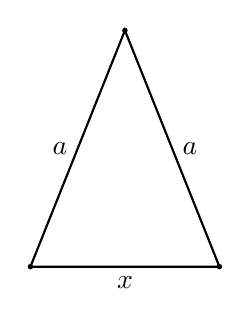
\begin{tikzpicture}[scale=1]
        \draw [line width=0.8pt]
              (-1.2, 0.0) -- node[below]{{\normalsize $x$}}
              ( 1.2, 0.0) -- node[right]{{\normalsize $a$}}
              ( 0.0, 3.0) -- node[left] {{\normalsize $a$}}
              (-1.2, 0.0);
        \fill (-1.2, 0.0) circle(1pt);
        \fill ( 1.2, 0.0) circle(1pt);
        \fill ( 0.0, 3.0) circle(1pt);
      \end{tikzpicture}
    \end{center}
  \fi
  %\ifoutline\outline\par
  %\fi
  %\ifoutcome\outcome\par
  %\fi
\end{exercise}
